\documentclass{article}

\usepackage{algorithmicx}
\usepackage{algpseudocode}
\usepackage{graphicx}
\usepackage{listings}
\usepackage{amsmath}
\usepackage{textcomp}
\usepackage{color}
\usepackage[%  
    colorlinks=true,
    pdfborder={0 0 0},
    linkcolor=blue
]{hyperref}

\lstset{ %
  language=Java,                  % the language of the code
  basicstyle=\footnotesize,       % the size of the fonts that are used for the code
  numbers=left,                   % where to put the line-numbers
  numberstyle=\tiny\color{gray},  % the style that is used for the line-numbers
  stepnumber=1,                   % the step between two line-numbers. If it's 1, each line
                                  % will be numbered
  numbersep=5pt,                  % how far the line-numbers are from the code
  backgroundcolor=\color{white},  % choose the background color. You must add \usepackage{color}
  showspaces=false,               % show spaces adding particular underscores
  showstringspaces=false,         % underline spaces within strings
  showtabs=false,                 % show tabs within strings adding particular underscores
  frame=single,                   % adds a frame around the code
  rulecolor=\color{black},        % if not set, the frame-color may be changed on line-breaks within not-black text (e.g. commens (green here))
  tabsize=4,                      % sets default tabsize to 2 spaces
  captionpos=b,                   % sets the caption-position to bottom
  breaklines=true,                % sets automatic line breaking
  breakatwhitespace=false,        % sets if automatic breaks should only happen at whitespace
  title=\lstname,                 % show the filename of files included with \lstinputlisting;
                                  % also try caption instead of title
  keywordstyle=\color{blue},          % keyword style
  commentstyle=\color{dkgreen},       % comment style
  stringstyle=\color{mauve},         % string literal style
  escapeinside={\%*}{*)},            % if you want to add a comment within your code
  morekeywords={*,...}               % if you want to add more keywords to the set
}


\title{Assignment Week 2 - Solutions}
\author{Course: Building Blocks of Programming}
\date{Topic: Flowcharts and operators}
\begin{document}
\maketitle

\begin{flushleft}

\textbf{Q 1. } Draw a flowchart that takes the attendance of three people as input 
(input will be 0 if they were absent and 1 if present) and displays whether all of 
them attended the class or not. Assume that the two values taken from input are 
always either 0 or 1.

\end{flushleft}

\begin{flushleft}

\textbf{Ans. } We can use the \lstinline{and} operator to check if all the students 
are present. Figure \ref{Q1} shows a sample flowchart.

\end{flushleft}

\begin{flushleft}

\textbf{Grading. } If the flowchart gives the correct grade then 2, if there are 
minor mistakes such as wrong boxes used for reading/printing then 1, otherwise 0.
This solution given is just one example, there are other valid solutions as well,
for example, we can also check whether \lstinline{a+b+c} is \lstinline{3}.

\end{flushleft}

\begin{figure}[ht]
    \centering
    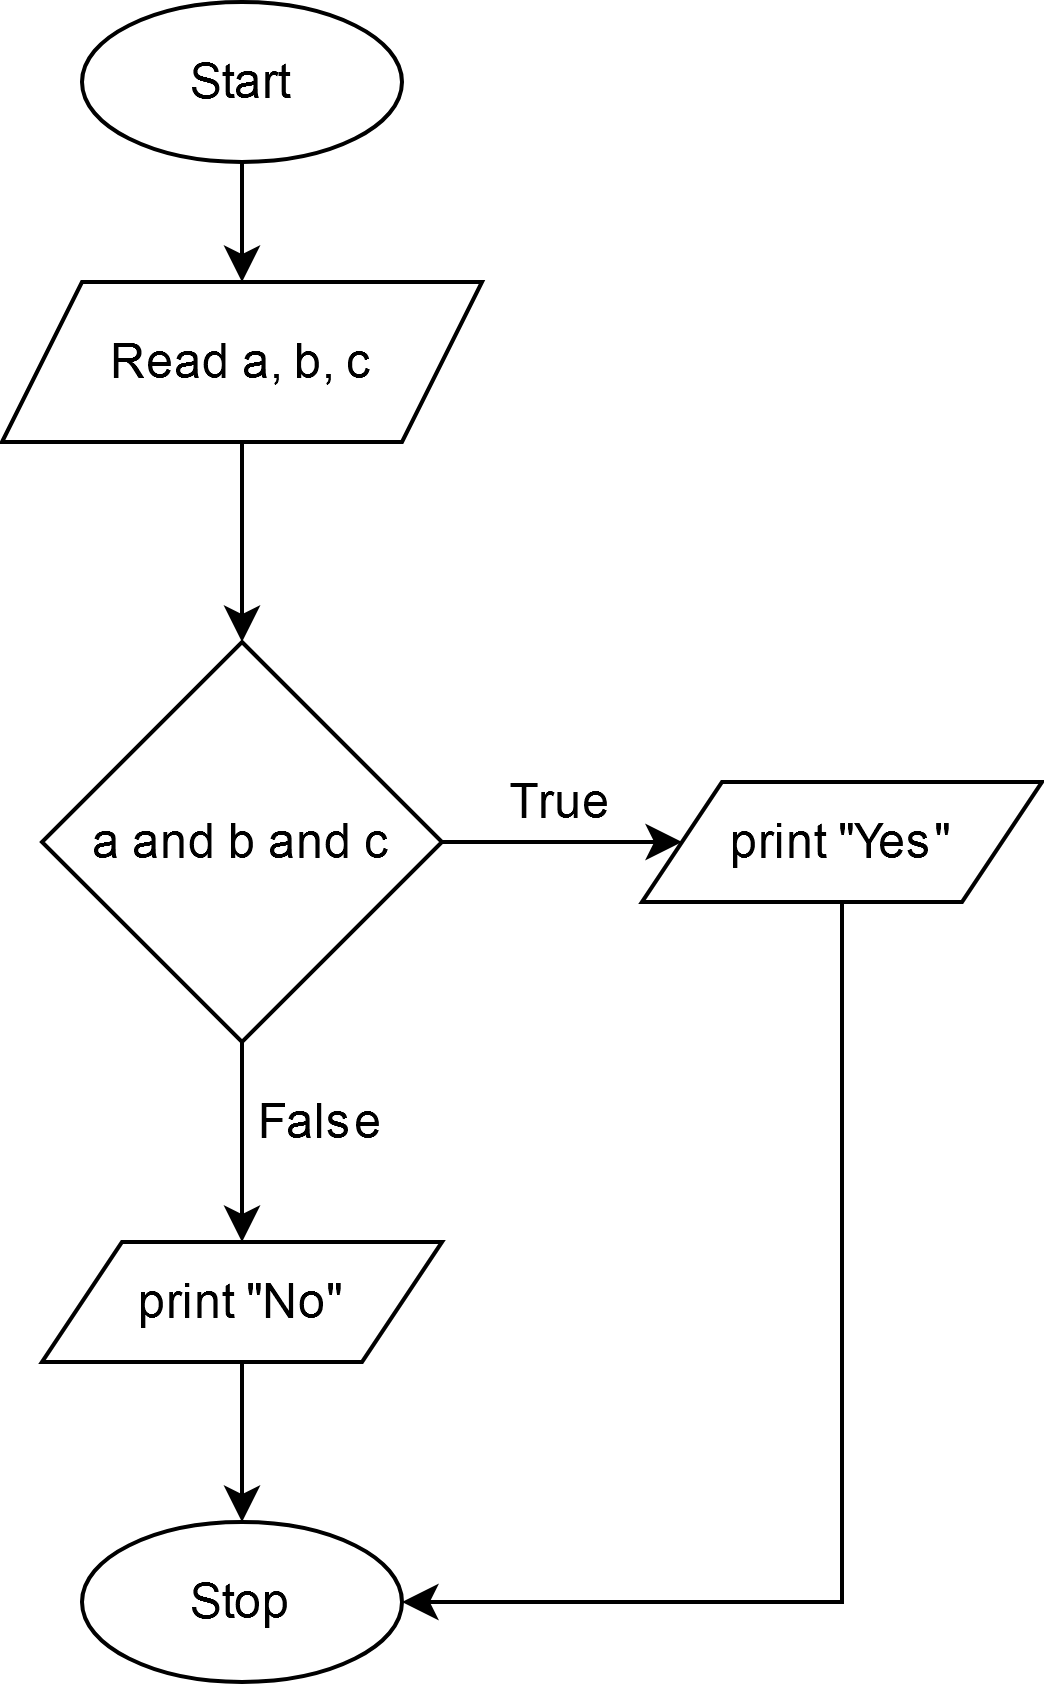
\includegraphics[width=0.5\textwidth]{Q1.png}
    \caption{Sample flowchart for Q1}
    \label{Q1}
\end{figure}

\clearpage

\begin{flushleft}

\textbf{Q 2.} Draw a flowchart that takes the score of a student as input and 
displays the grade of the student as follows

\begin{itemize}
    \item $\text{score} \geq 90$ receives A+
    \item $90 > \text{score} \geq 80$ receives A
    \item $80 > \text{score} \geq 70$ receives B+
    \item $70 > \text{score} \geq 60$ receives B
    \item $60 > \text{score} \geq 50$ receives C+
    \item $50 > \text{score} \geq 40$ receives C
    \item $\text{score} < 40$ receives D
\end{itemize}

\end{flushleft}

\begin{flushleft}

\textbf{Ans. } We can use if statements and comparators to find the range of the 
input variable. Sample solution is in Figure \ref{Q2}

\begin{figure}[ht]
    \centering
    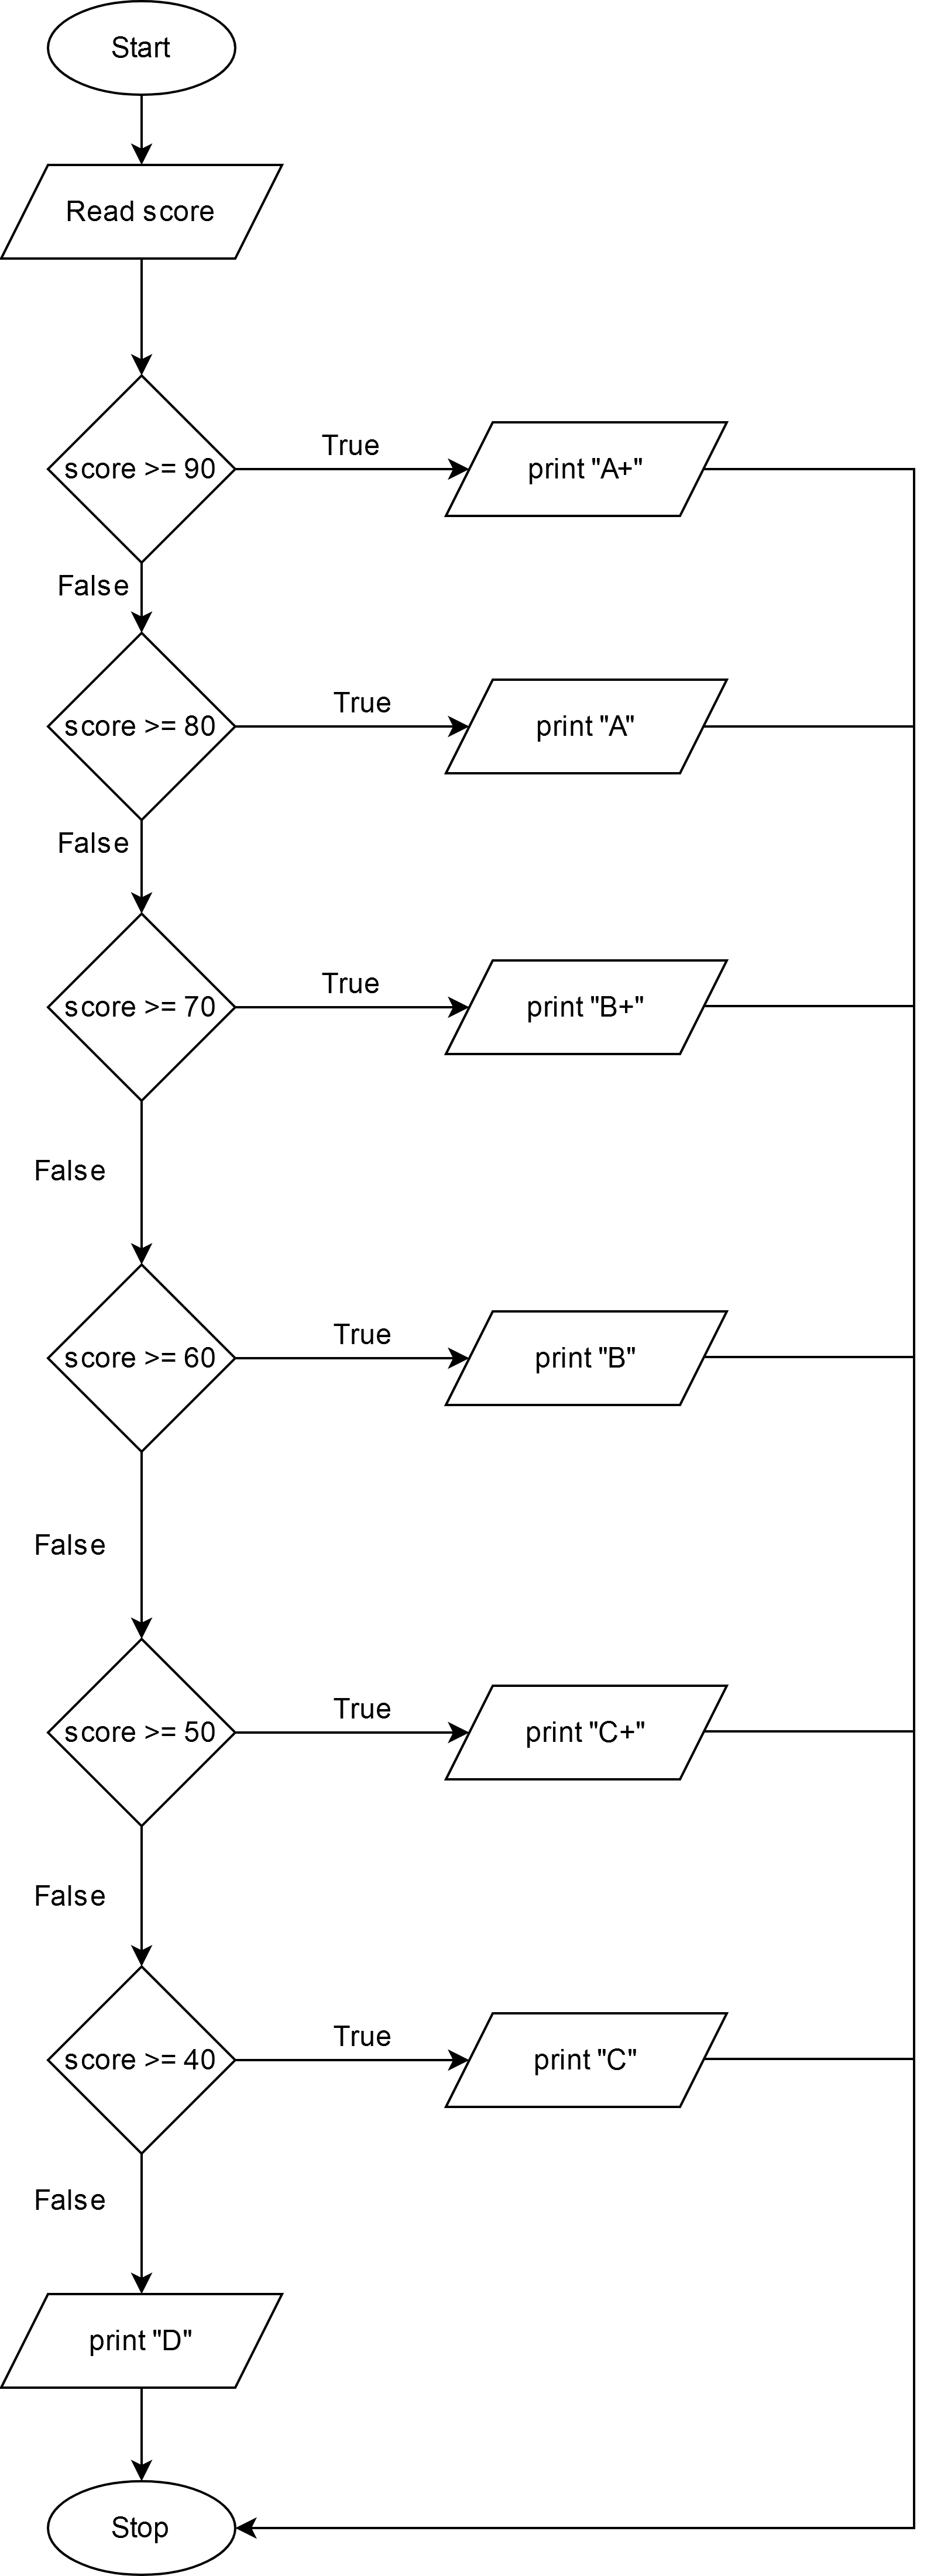
\includegraphics[width=0.5\textwidth]{Q2.png}
    \caption{Sample flowchart for Q2}
    \label{Q2}
\end{figure}

\end{flushleft}

\begin{flushleft}
\textbf{Grading. } If the flowchart gives the correct output then 2, if there are 
minor mistakes such as wrong boxes used for reading/printing then 1, otherwise 0.

The solution given is just one example, there could be other equivalent valid 
flowcharts.
\end{flushleft}

\clearpage

\begin{flushleft}

\textbf{Q 3.} Draw a flowchart for finding the maximum of 4 numbers which are 
obtained as input from the user. Print “maximum value = \textlangle the maximum number\textrangle“ 
at the end.

\end{flushleft}

\begin{flushleft}

\textbf{Ans. } Simple extension of the question discussed in class.
We can just add another comparison between the result obtained for three variables and
the last variable. Alternatively we can store another variable that contains the answer
and update it, this is shown in Figure \ref{Q3}.

Note: You cannot use less than 3 comparisons to solve this question. For obtaining the
minimum/maximum of $n$ numbers we need at least $n-1$ comparisons. 

\end{flushleft}

\begin{flushleft}

\textbf{Grading. } If the flowchart gives the correct output then 2. Not following
the output specifications or not printing the maximum value is not penalised,
as long as the maximum value is obtained correctly using conditional statements,
give 2. If there are errors in the flowchart, that is wrong boxes are used, but the
overall logic/intention of the flowchart is correct then 1, otherwise 0.
        
\end{flushleft}

\begin{figure}[ht]
    \centering
    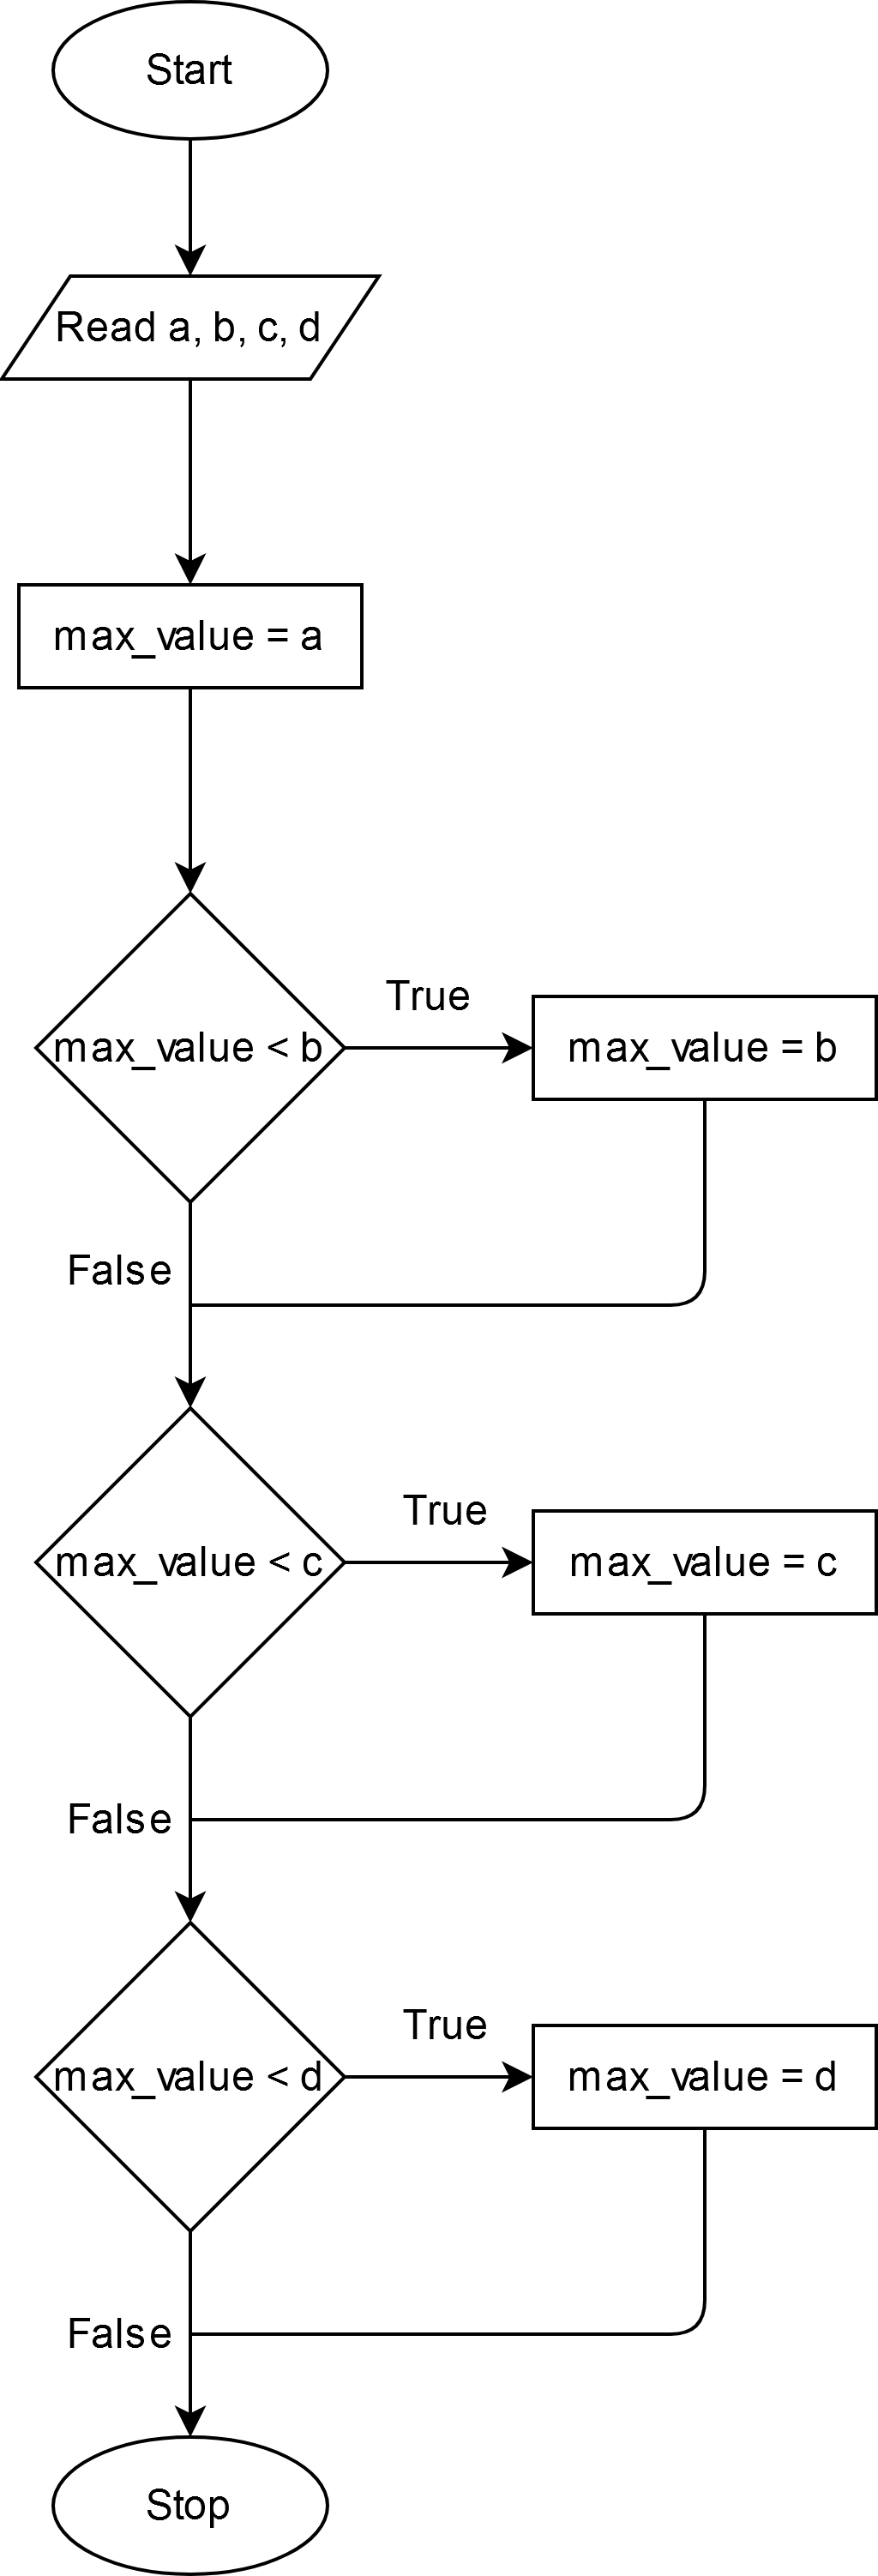
\includegraphics[width=0.5\textwidth]{Q3.png}
    \caption{Sample flowchart for Q3}
    \label{Q3}
\end{figure}

\clearpage

\begin{flushleft}

\textbf{Q 4.} Draw a flowchart that takes an integer, the year as input and 
displays “yes” if the year is a leap year and “no” otherwise.
Note : Please refer 
\href{https://en.wikipedia.org/wiki/Leap_year#Algorithm}{Wikipedia} for the exact 
criteria to determine if a given year is a leap year.

\end{flushleft}

\begin{flushleft}

\textbf{Ans. } Simply implement the algorithm given in Wikipedia using conditional
operators. There are multiple ways to draw a flowchart, one example is given in 
Figure \ref{Q4}.

\end{flushleft}

\begin{flushleft}

\textbf{Grading. } If the output of the flowchart is correct then 2, if there are 
errors in the flowchart (such as incorrect boxes being used for reading input/output)
then 1, otherwise 0.
    
\end{flushleft}

\begin{figure}[ht]
    \centering
    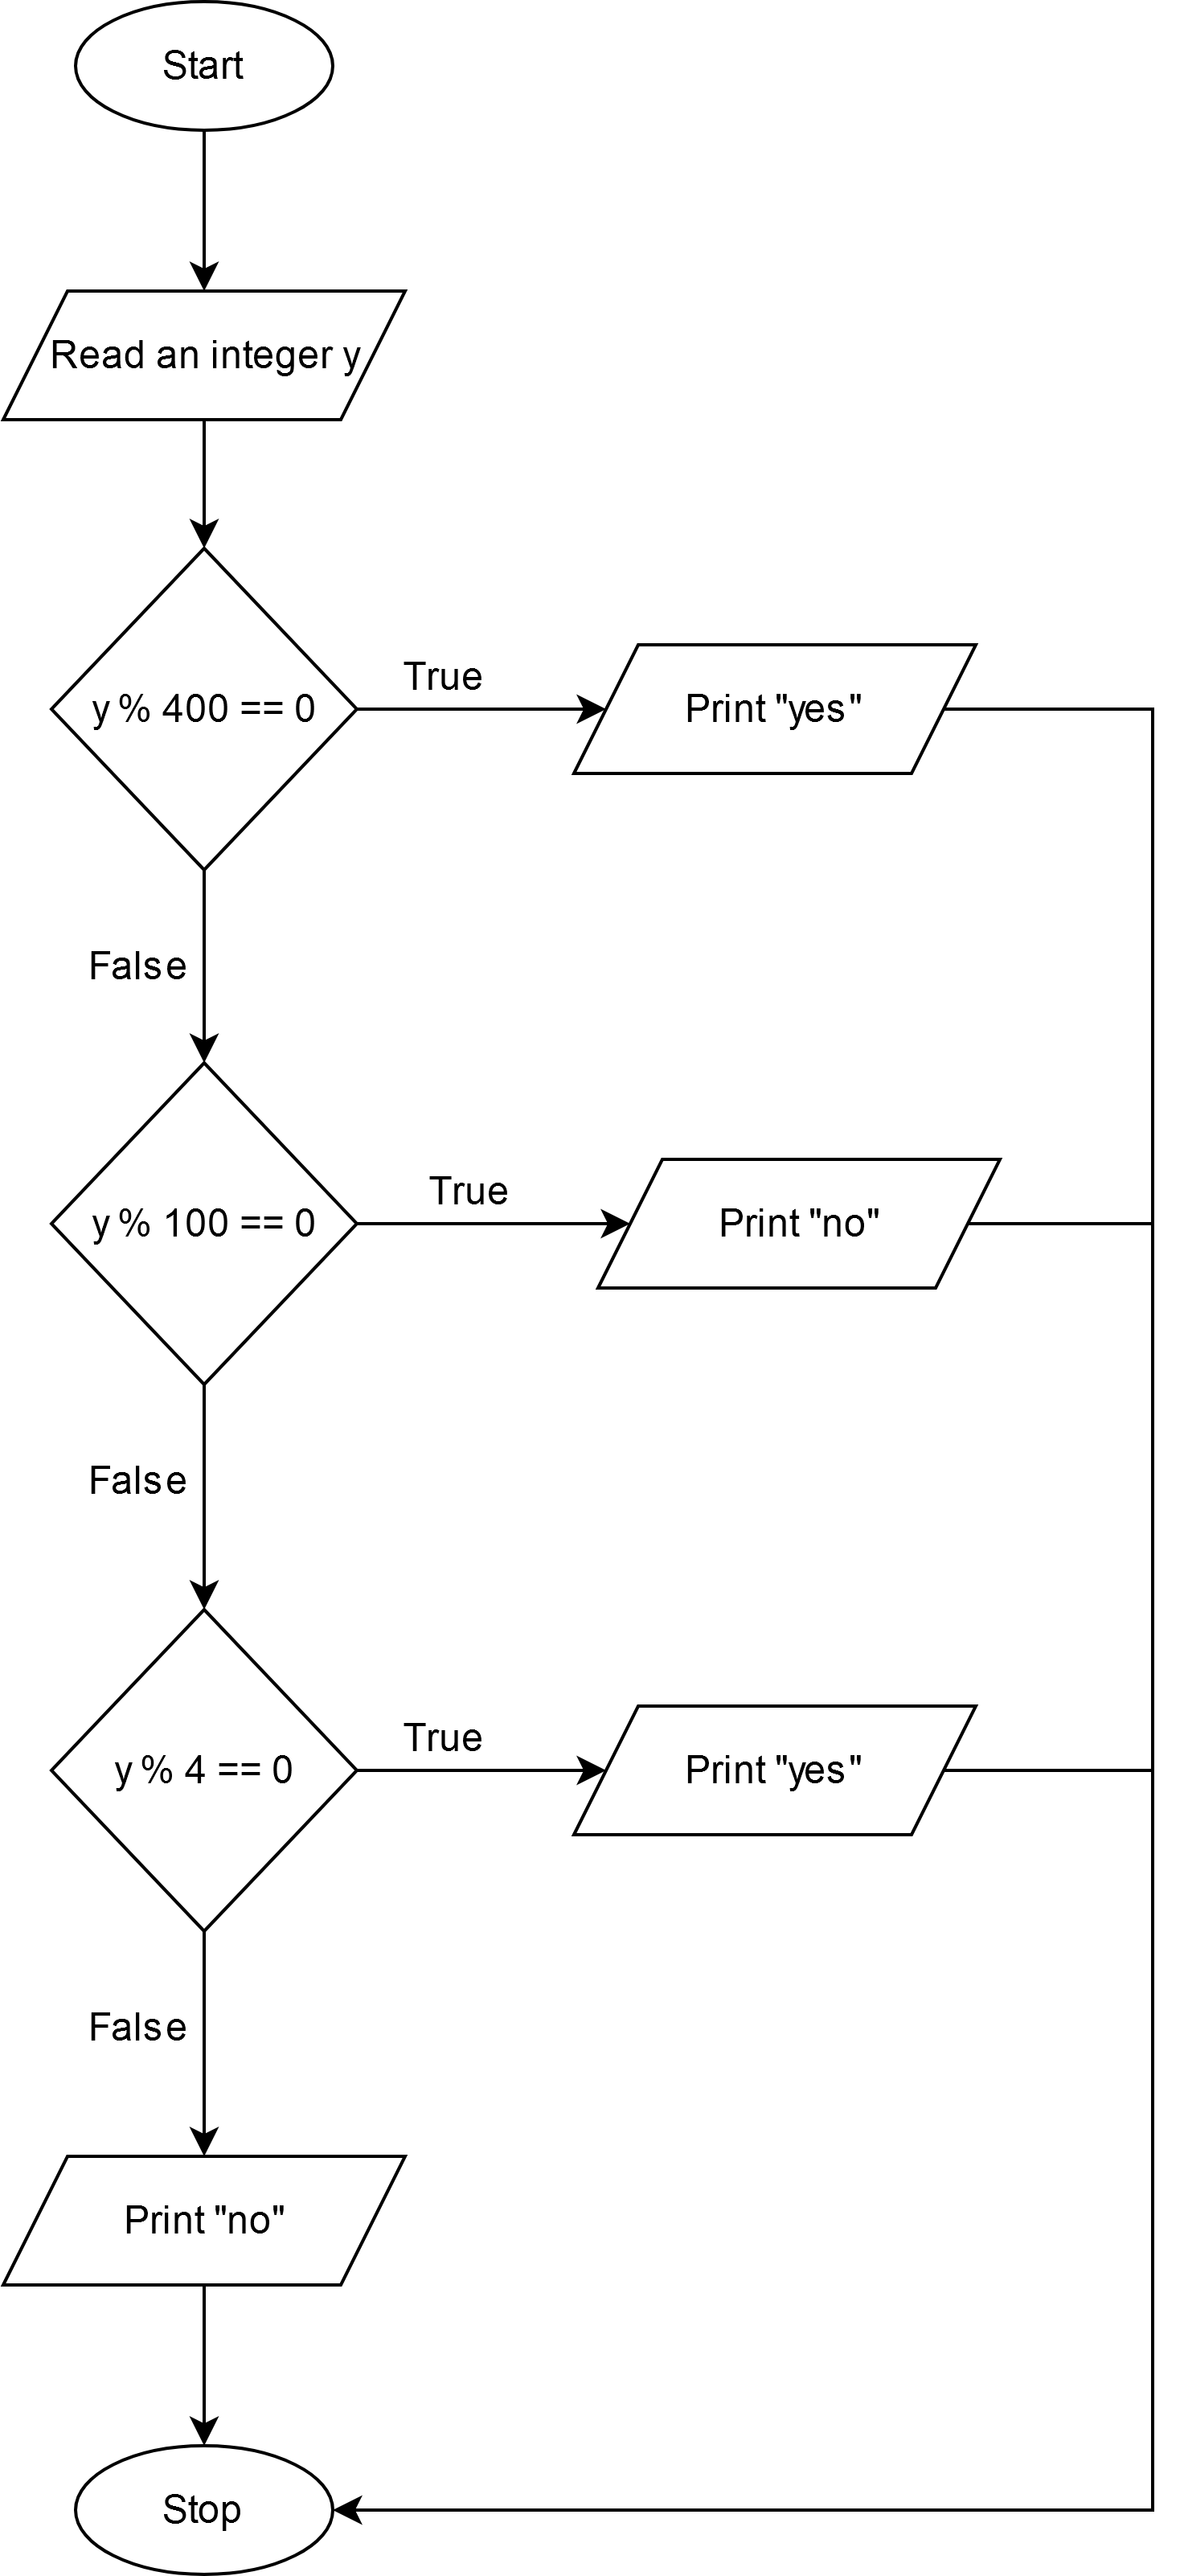
\includegraphics[width=0.5\textwidth]{Q4.png}
    \caption{Sample flowchart for Q4}
    \label{Q4}
\end{figure}

\clearpage

\begin{flushleft}

\textbf{Q 5. } Draw a flowchart that takes the three angles of a triangle (in degrees)
as input and prints whether the triangle is acute, right-angled, obtuse or invalid 
(i.e. a triangle with such angles does not exist). Assume that the 3 numbers obtained 
from input are \textbf{positive} real numbers.
    
\end{flushleft}


\begin{flushleft}

\textbf{Ans. } Suppose the angles are \lstinline{a, b, c} then the triangle will be 
valid if and only if \lstinline{a + b + c == 180}. Note that since the angles are 
guaranteed to be positive, this condition is sufficient to say that the triangle is 
valid.

A triangle is obtuse if any angle is greater than 90.

A triangle is right-angled if one of the angles is equal to 90.

If a triangle is valid and it is not obtuse or right angled then it must be acute.

This solution is shown in Figure \ref{Q5}. Several other solutions exist, for example,
we can check if a triangle is acute by checking if all angles are less than 90.
    
\end{flushleft}

\begin{flushleft}

\textbf{Grading. } If flowchart gives the correct output then 2, if the logic is correct,
but there are mistakes in the flowchart then 1, otherwise 0.
        
\end{flushleft}

\begin{figure}[ht]
    \centering
    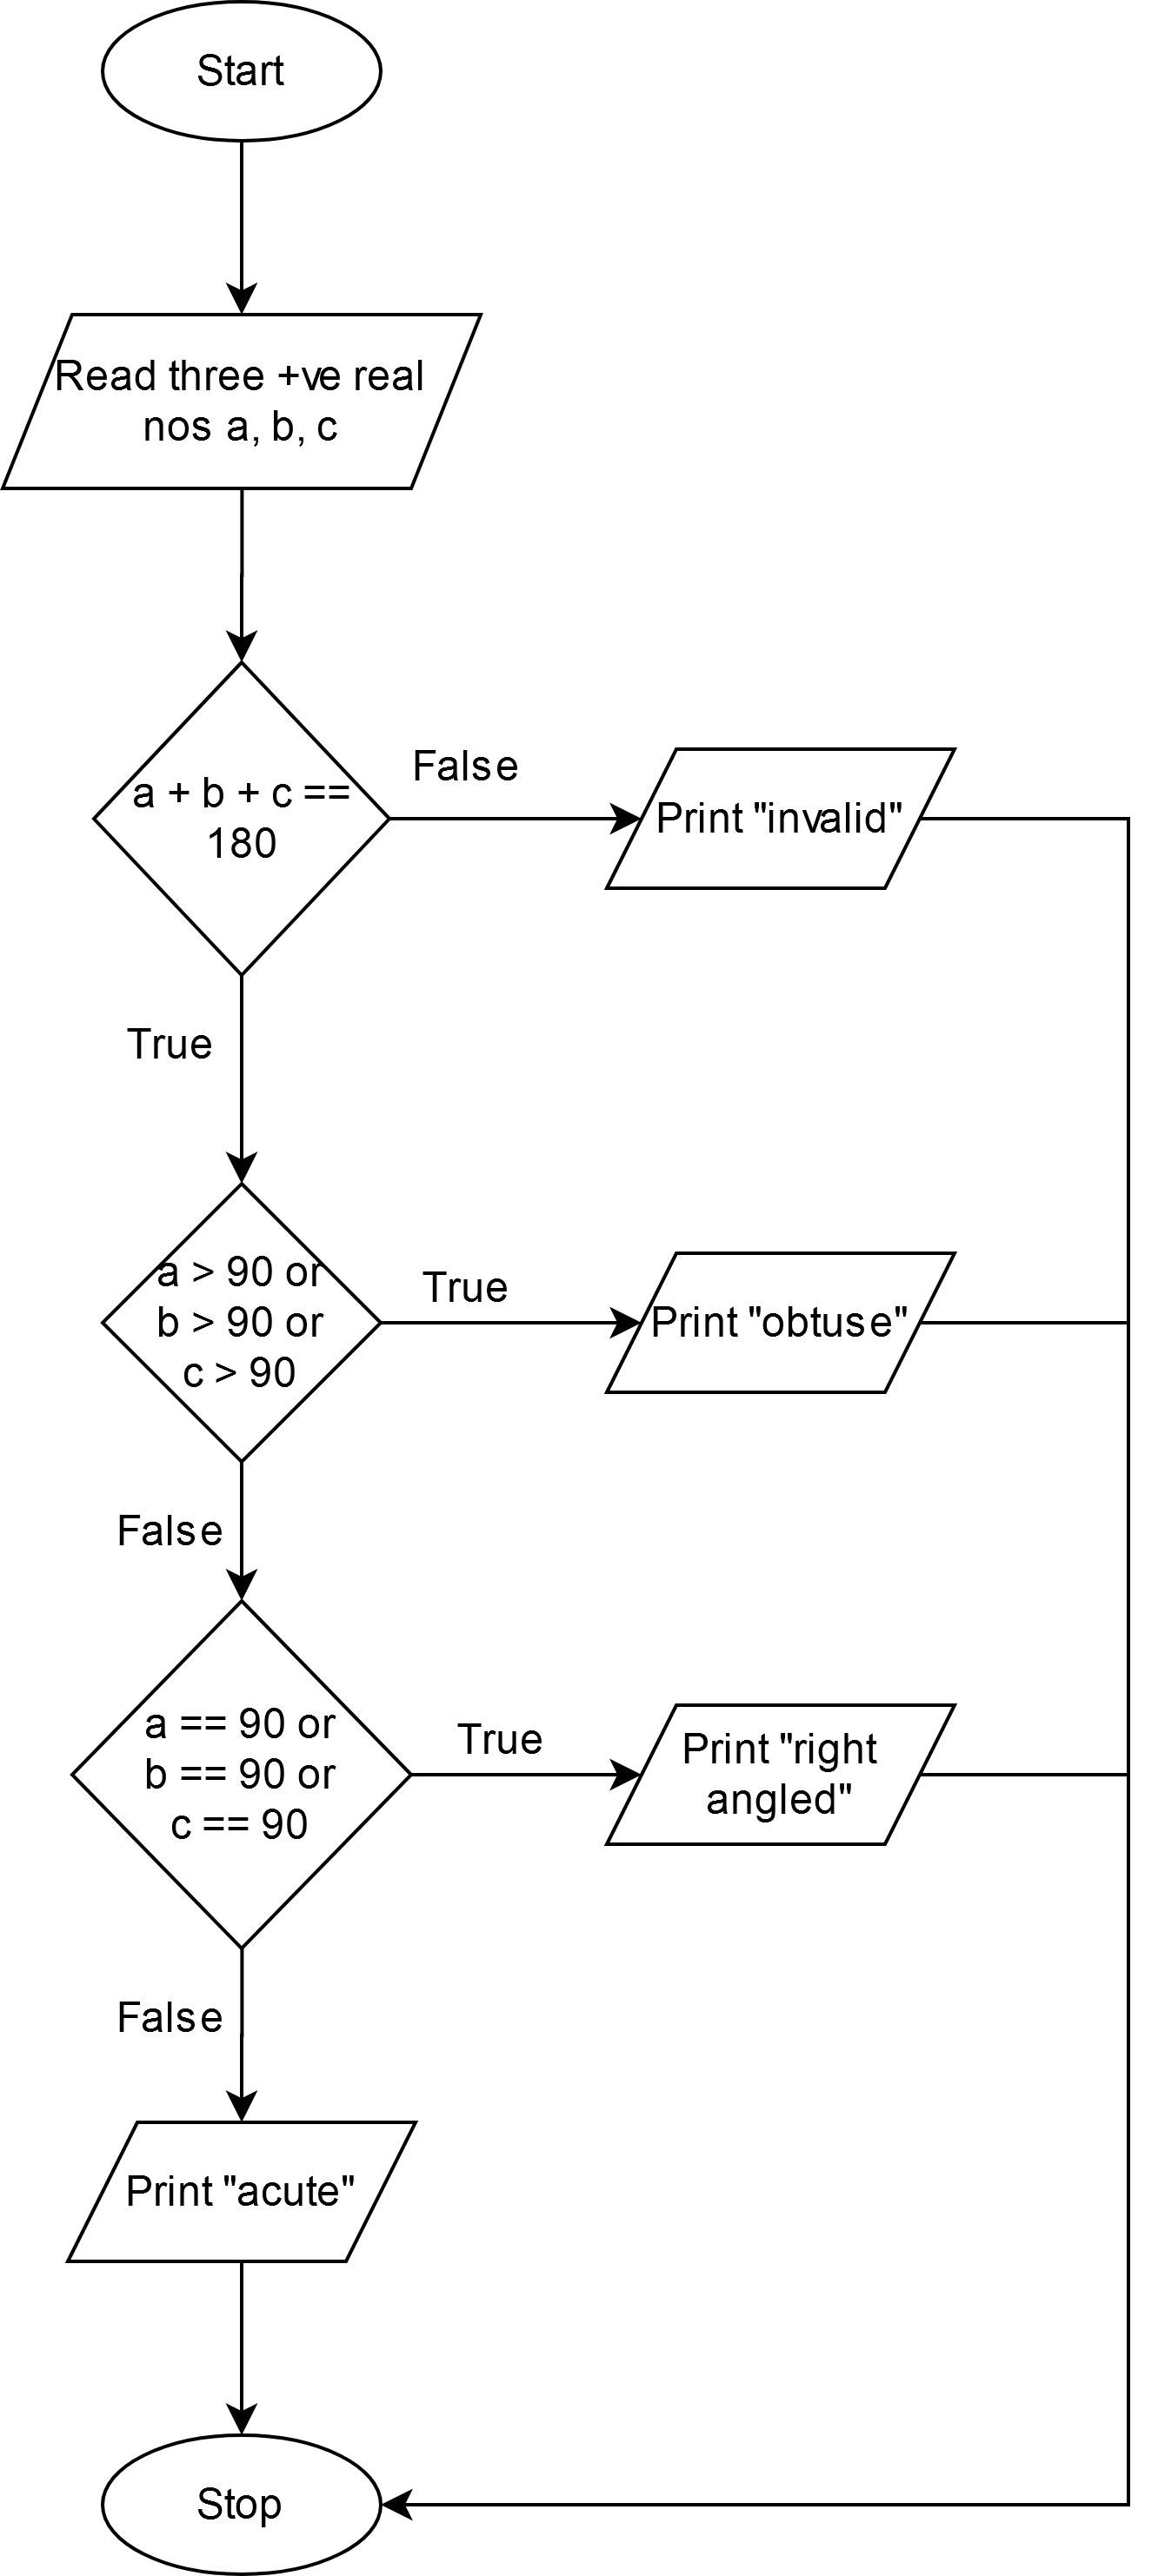
\includegraphics[width=0.5\textwidth]{Q5.png}
    \caption{Sample flowchart for Q5}
    \label{Q5}
\end{figure}

\clearpage

\begin{flushleft}

\textbf{Q 6. } Draw a flowchart that takes the perimeter and area of a rectangle as 
input and displays whether such a rectangle exists or not. Assume that the perimeter and
area taken from input are positive real numbers. (Note: You should use only the operators
that you have learned, i.e. +, -, *, /, //, **, and, or, not, xor, $>$, $<$, $==$, $>=$, $<=$ and $!=$).
    
\end{flushleft}

\begin{flushleft}

\textbf{Ans. } Let $p, A$ denote the perimeter and the area of the rectangle respectively.

If $a, b$ are the sides of the rectangle then $a + b = \frac{p}{2}$ and $ab = A$

Therefore $a, b$ are roots of the quadratic equation $X^2 - \frac{p}{2}X + A = 0$.

Since $p, A$ are positive numbers, as long as there exists a solution to the quadratic equation, 
both the solutions will be positive, so the only condition that we need to check is that the 
discriminant of the quadratic equation is non-negative.

This gives $\frac{p^2}{4} \geq 4A \implies p^2 \geq 16 A$ described in Figure \ref{Q6}

Other equivalent solutions may exist. In the original question, the relational operators
were missed, but they were intended to be allowed. The intention was to not allow the use 
of $\sqrt{x}$ in the flowchart, however "** 0.5" can be used instead, although it is not required. 
Sorry for the error.

\end{flushleft}

\begin{flushleft}

\textbf{Grading. } If the flowchart gives the correct output then 2. If the condition derived is 
correct but there are errors in the flowchart then 1, otherwise 0.
        
\end{flushleft}

\begin{figure}[ht]
    \centering
    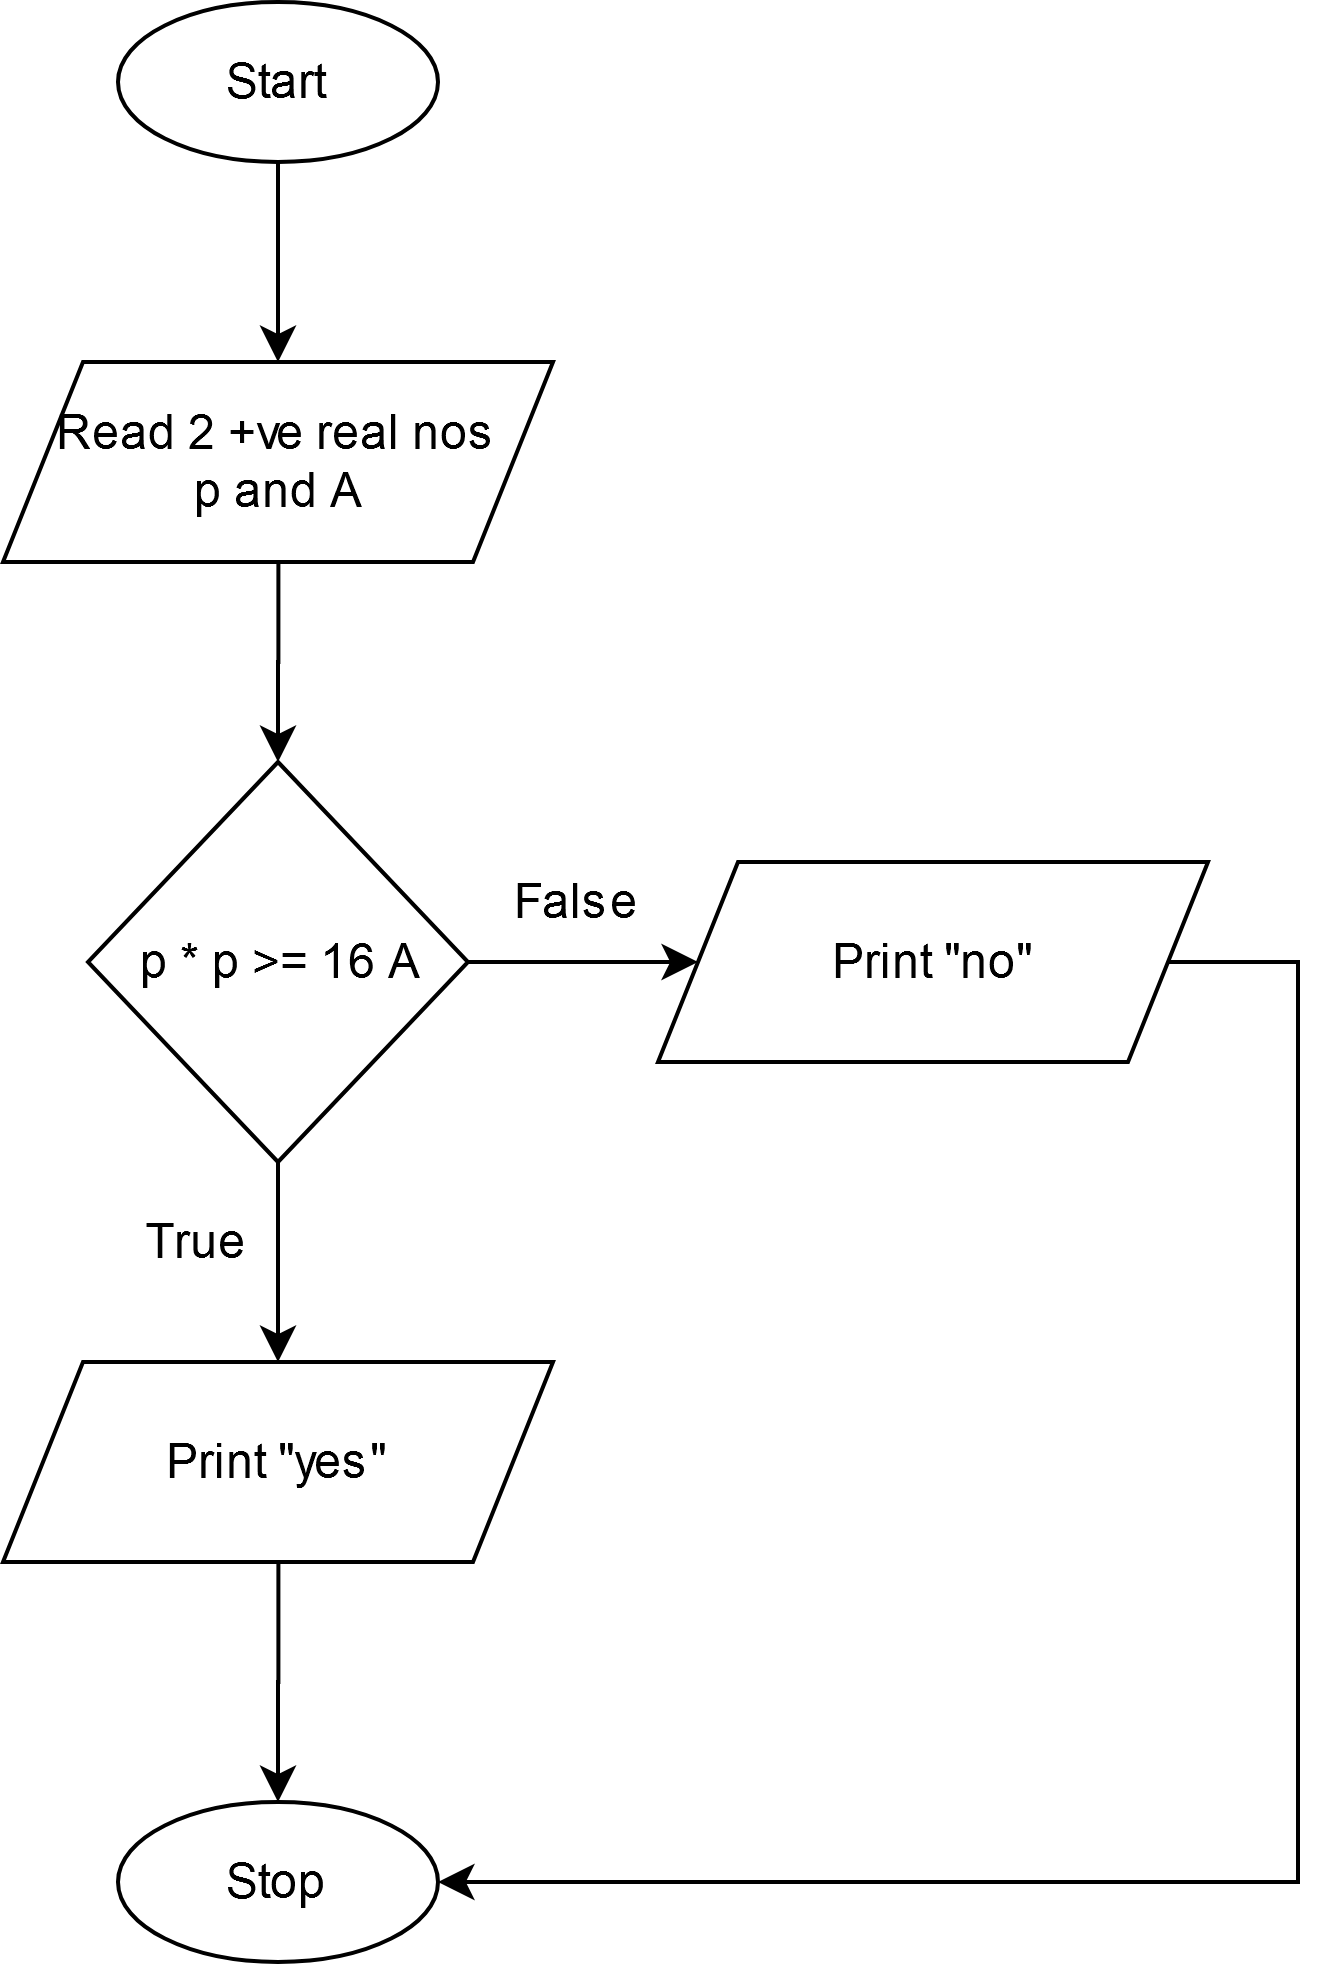
\includegraphics[width=0.5\textwidth]{Q6.png}
    \caption{Sample flowchart for Q6}
    \label{Q6}
\end{figure}

\clearpage

\begin{flushleft}

\textbf{Q 7. } Draw a flowchart for the color of light to be displayed at a traffic signal, 
by reading as input the current time $t$, the signal switching time $s$ and transition time $u$. 
Assume that

\begin{itemize}
    \item The color at $t = 0$ is red 
          (remains red from $t=0$ to $s-1$)
    \item After $s$ seconds (i.e. at $t=s$) color changes to yellow
          (remains yellow from $t=s$ to $s+u-1$)
    \item After another $u$ seconds (i.e. at $t=s+u$)  the color changes to green
          (remains green from $t=s+u$ to $2s+u-1$)
    \item After another $s$ seconds (i.e. at $t=2s+u$) the color changes to yellow
          (remains yellow from $t=2s+u$ to $2s+2u-1$)
    \item After another $u$ seconds  (i.e. at $t=2s+2u$) the color changes back to red, 
          which is displayed for $s$ seconds and the cycle continues
          (remains red from $t=2s+2u$ to $3s+2u-1$)
\end{itemize}

Note that red and green are displayed for $s$ seconds, and yellow for $u$ seconds.

Assume all input variables $t, s, u$ are \textbf{positive} integers.
Print the color to be displayed at the end.

\end{flushleft}

\begin{flushleft}

\textbf{Ans. } We can see that the colors displayed repeats every $2s + 2u$ seconds. 

So the color at a certain time $t$ will be equal to the color at time $t \% (2s + 2u)$.

Let $r = t \% (2s + 2u)$, we know that $0 \leq r < 2s+2u$. So $r$ will fall in one of the four 
cases that were already mentioned in the question. The flowchart is in Figure \ref{Q7}.
    
\end{flushleft}

\begin{figure}[ht]
    \centering
    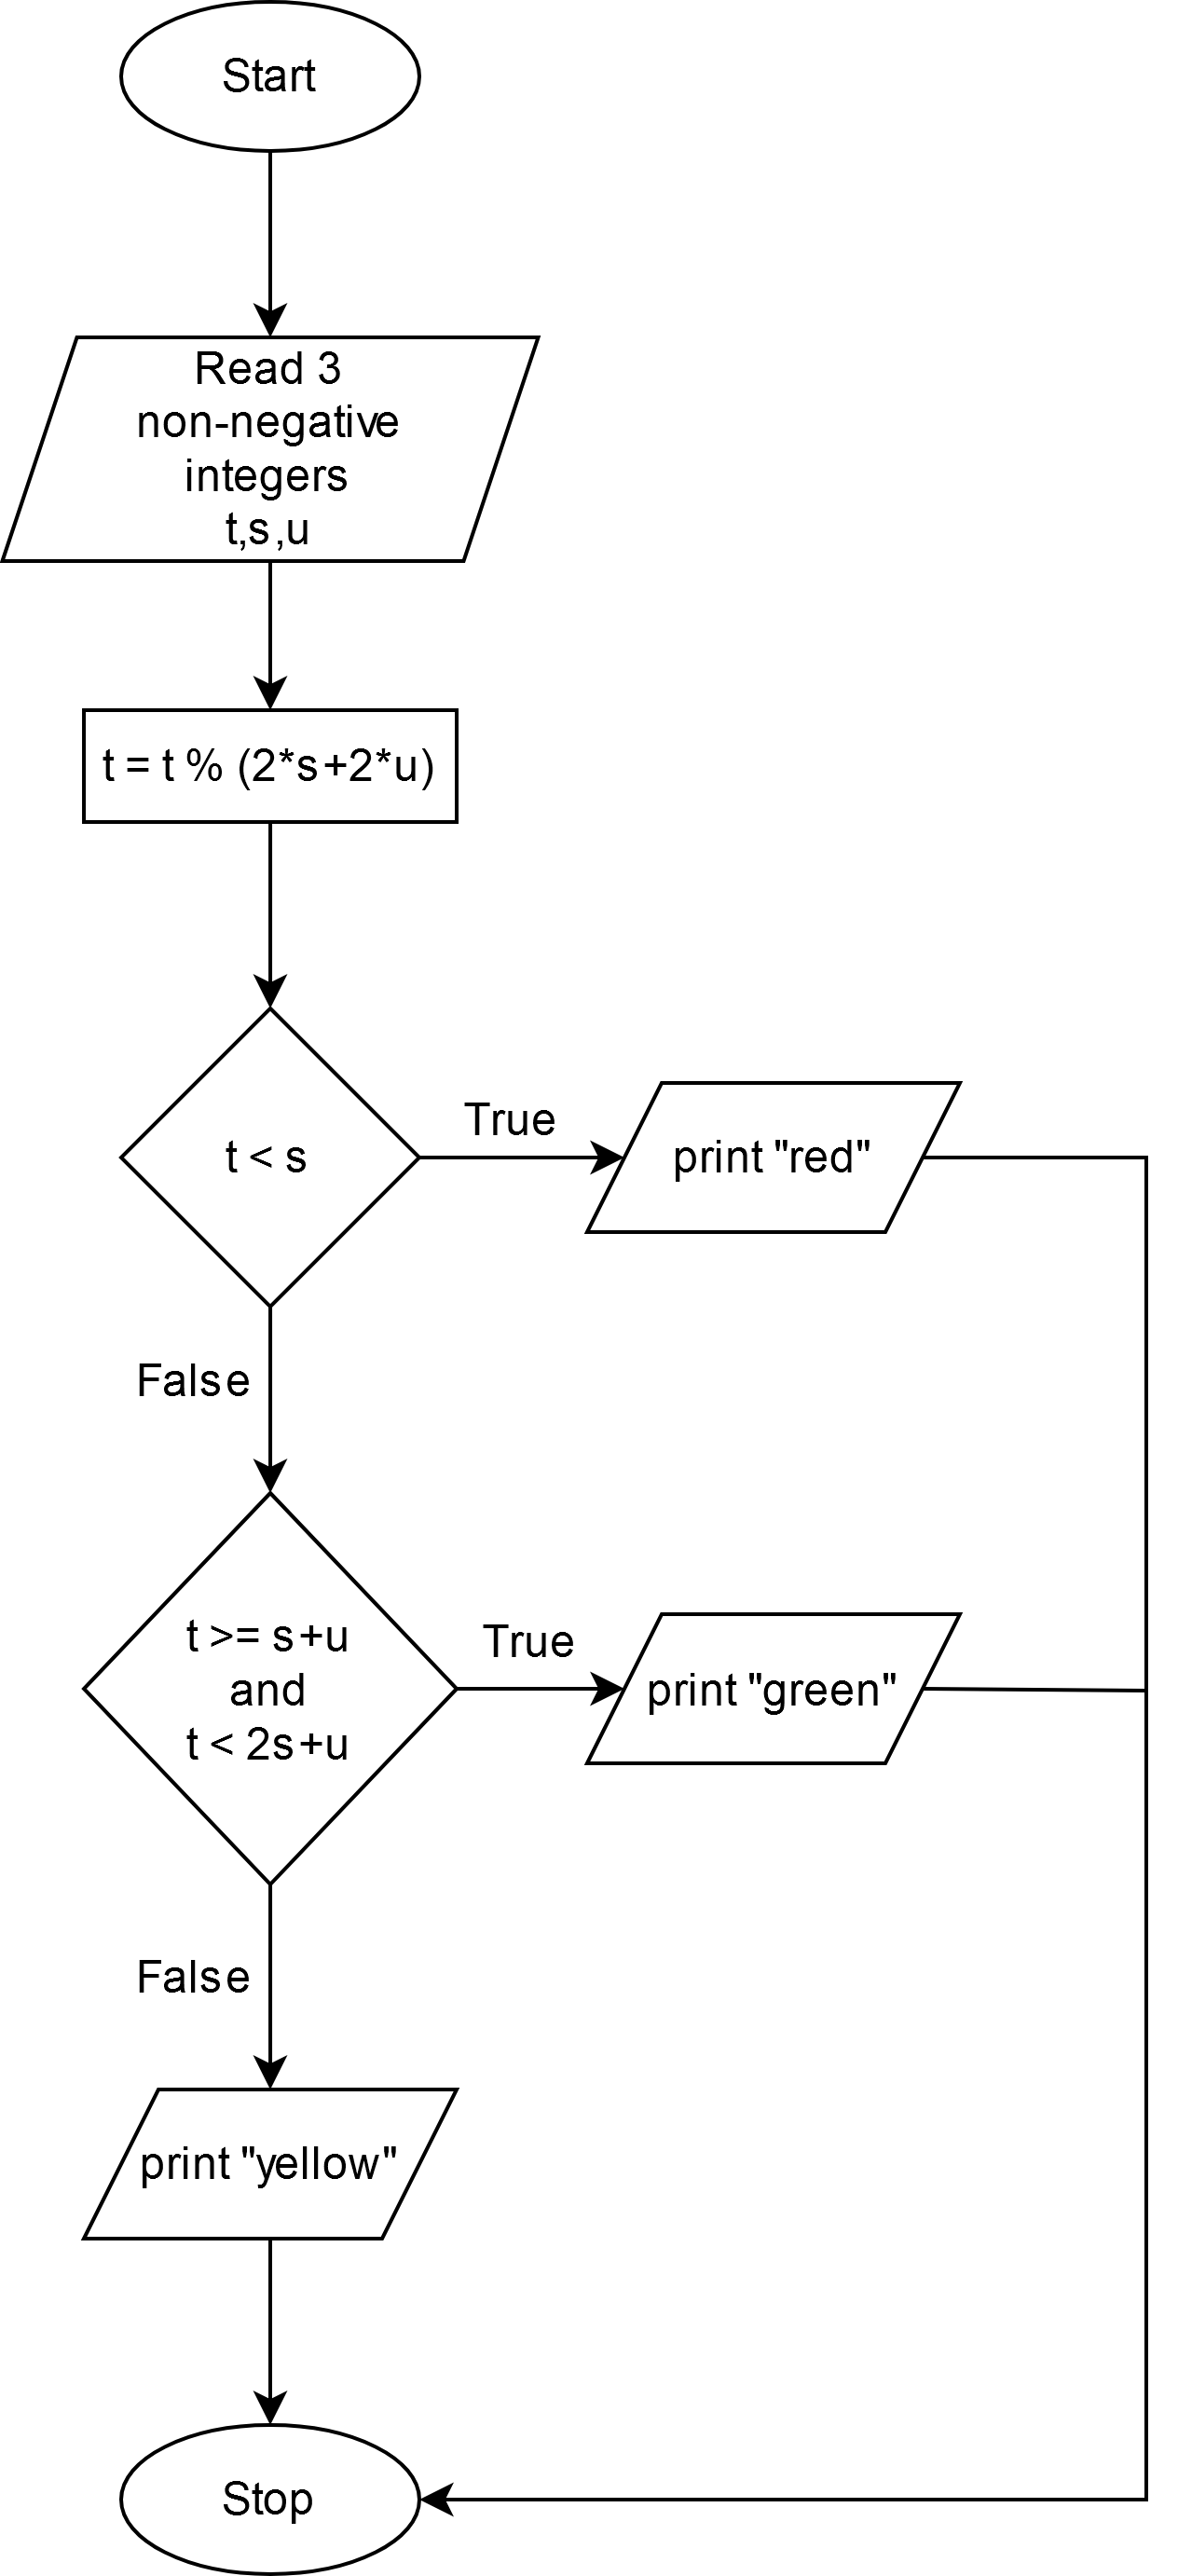
\includegraphics[width=0.5\textwidth]{Q7.png}
    \caption{Sample flowchart for Q7}
    \label{Q7}
\end{figure}

\begin{flushleft}

\textbf{Grading. } If the flowchart is correct then 2, if the logic is correct but there are 
mistakes in the drawing of the flowchart or any operations then 1, otherwise 0.

\end{flushleft}
    
\clearpage

\begin{flushleft}

\textbf{Q 8. } For any two positive integers $x, y$ explain why there exists a unique pair of 
integers $q, r$ which satisfies 

\begin{itemize}
    \item $y = x q + r$
    \item $0 \leq r < x$
\end{itemize}

Also show how to obtain the integers $q, r$ from $x, y$ using the operators that you have learned
(+, -, *, /, //, **, \%)
    
\end{flushleft}

\begin{flushleft}

\textbf{Ans. } Suppose there existed more than one pair, let them be $q_1, r_1$ and $q_2, r_2$
\linebreak
Then $y = q_1 x + r_1$ and $y = q_2 x + r_2$.
\linebreak
Subtracting the two equations we get $r_2 - r_1 = (q_1 - q_2) x \implies r_2 - r_1 \text{is a multiple of }x$
\linebreak
Since $0 \leq r_1, r_2 < x$, we have $-x < r_1 - r_2 < x$.
The only multiple of $x$ strictly between $-x, x$ is $0$, therefore, $r_1 - r_2 = 0$ which implies 
that $r_1 = r_2$ and $q_1 = q_2$. This is a contradiction and hence proves the statement.
\linebreak
To obtain $q, r$ we observe that when we divide $y$ by $x$, we obtain a quotient $q$ and remainder $r$ that 
satisfies both conditions given. So $r = y \% x$ and $q = y // x$.
\linebreak
We can also write $r$ as $y - x * (y // x)$ and $q$ as $(y - (y \% x)) / x$.
\linebreak
Note: "$\%$" was missed when listing down the operations in the original question, however it was intended to be allowed. 
Although it is possible to express using only //, solutions which use "$\%$" will also be considered
correct.
Sorry for the error.
    
\end{flushleft}

\begin{flushleft}

\textbf{Grading. } A formal proof as given is not required. If the expressions for $q, r$ are correctly 
obtained then 2, if the expressions for $q, r$ are not correct and the explanations for unique pair are 
reasonable then 1, otherwise 0.
        
\end{flushleft}

\clearpage

\begin{flushleft}

\textbf{Q 9. } List down the values of the units digit of the first 10 powers of 3. In other words calculate
$(3^x) \% 10$ for $x = 0, 1, \ldots 9$. Observe the pattern and draw a flowchart to calculate $(3^x) \% 10$
where $x$ is any \textbf{non-negative} integer which is obtained as input. 

\end{flushleft}

\begin{flushleft}

\textbf{Ans.} The unit digits of the first 10 powers of 3 are $1, 3, 9, 7, 1, 3, 9, 7, 1, 3$. We can clearly 
see the pattern that $1, 3, 9, 7 \ldots$ repeats. We can prove this by observing that 
$(x * y) \% 10 = ((x \% 10) * (y \% 10)) \% 10$. So once any number repeats in the sequence from that point 
the unit digits will start repeating. In this case we see that $1, 3, 9, 7$ will repeat.

So we can find $(3^x) \% 10$ by the following formula

\begin{itemize}
    \item $x \% 4 == 0 \implies $ unit digit is $1$  
    \item $x \% 4 == 1 \implies $ unit digit is $3$  
    \item $x \% 4 == 2 \implies $ unit digit is $9$  
    \item $x \% 4 == 3 \implies $ unit digit is $7$  
\end{itemize}

The flowchart is shown in Figure \ref{Q9}.

\textbf{Grading.} If flowchart is correct (even if it is correct only for the first 10 powers) then 2, 
if the flowchart is not correct but the unit digits were identified correctly then 1, otherwise 0.

\end{flushleft}

\begin{figure}[ht]
    \centering
    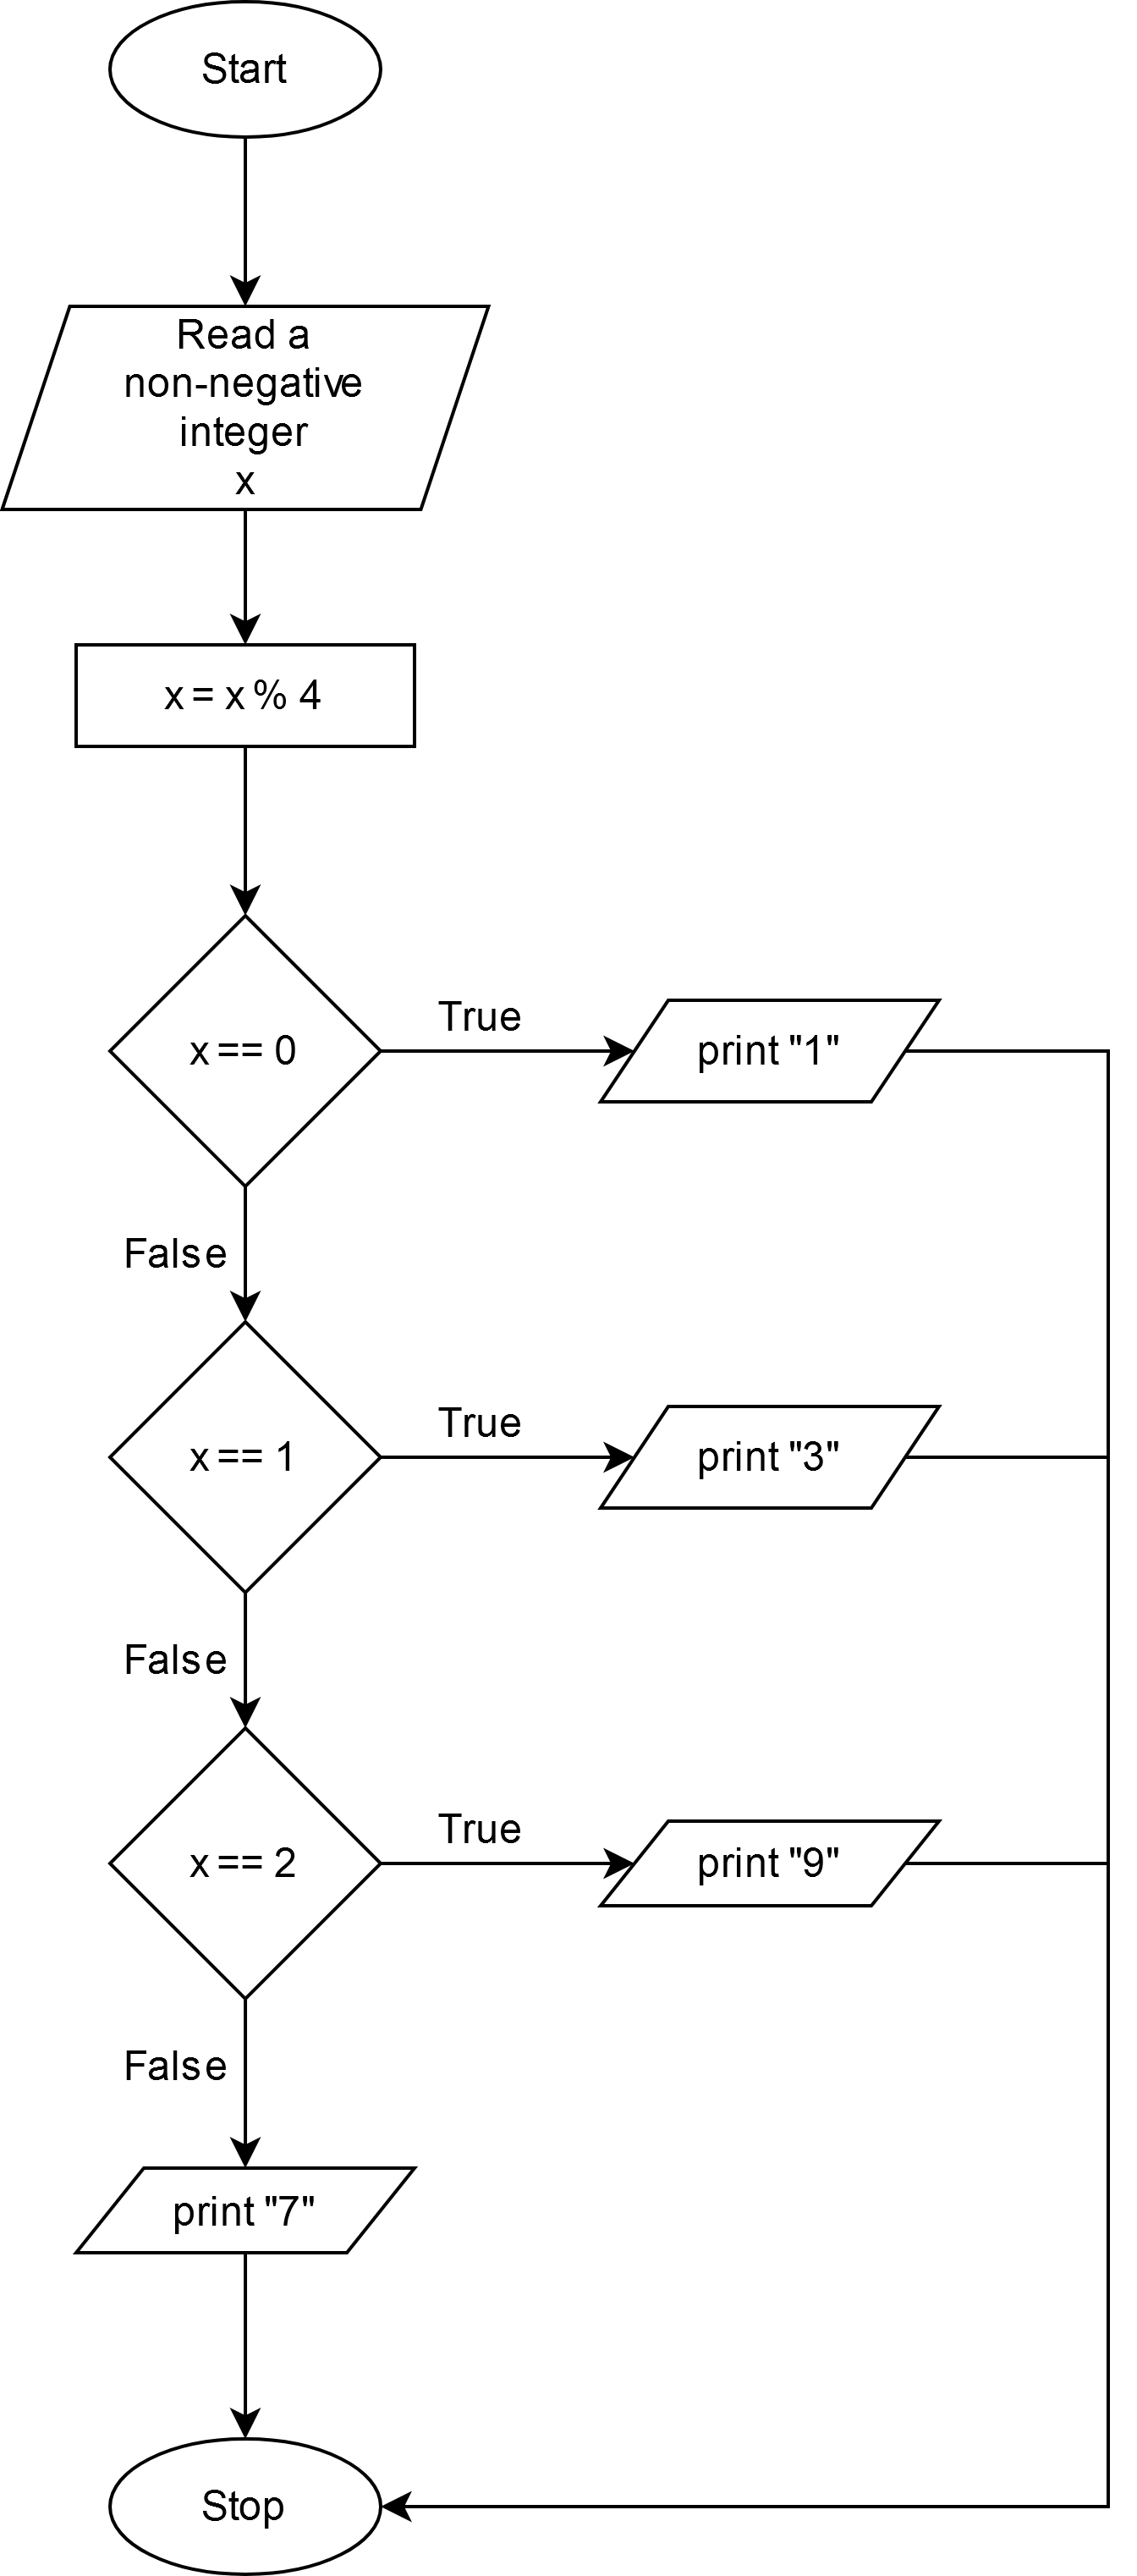
\includegraphics[width=0.5\textwidth]{Q9.png}
    \caption{Sample flowchart for Q9}
    \label{Q9}
\end{figure}


\clearpage

\begin{flushleft}

\textbf{Q 10. } Explain why the following statement is true (or provide a counterexample if it is false) 
\linebreak
\textbf{Statement.} For any two positive integers $x, y$, the value of $x \% y$ (i.e. the remainder when 
$x$ is divided by $y$) is either equal to $x$ or less than or equal to $\frac{x}{2}$.

\end{flushleft}

\begin{flushleft}

\textbf{Ans. } We consider 3 cases, 
\linebreak
\textbf{Case 1.} $x < y$: 
\linebreak
In this case $x \% y = x$ and so the statement is true
\linebreak
\textbf{Case 2.} $x \geq y$ and $y \leq \frac{x}{2}$: 
\linebreak
Since $x \% y < y$ and $y \leq \frac{x}{2}$ we can conclude that 
$x \% y < \frac{x}{2}$ and so the statement is true
\linebreak
\textbf{Case 3.} $x \geq y$ and $y > \frac{x}{2}$: 
\linebreak
Since $x \geq y$, $q \geq 1$ where $q = x // y$. 
We know that $x = y q + (x \% y) \implies x \% y = x - y q \leq x - y < x - \frac{x}{2} < \frac{x}{2}$
\linebreak
In the three cases we have covered all possible values for the pair $x, y$ and hence the statement is true.
\end{flushleft}

\begin{flushleft}

\textbf{Grading. } If correct reasoning is provided then 2, otherwise if it is identified that the statement
is true and an attempt has been made at some reasoning then 1, otherwise 0.
    
\end{flushleft}

\end{document}